\documentclass{beamer}
\usepackage{asymptote}
\usepackage[french]{babel}
\usepackage[utf8]{inputenc}
\usepackage[T1]{fontenc}
\usepackage{lmodern}
\usepackage{enumerate}
\usepackage{amsmath, amssymb, amsthm}
% for use in integrals and derivatives
\newcommand{\dd}{\mathrm d}
\usepackage{hyperref}
\usetheme{Warsaw}
\usefonttheme{professionalfonts}
\setbeamertemplate{navigation symbols}{}
\setbeamertemplate{headline}{}

\title{Le modèle de Thomas-Fermi-von Weizs\"acker ultra-relativiste}
\author{Gaspard Jankowiak et Antoine Levitt}
\date{24 mars 2011}
\institute{Groupe de travail des thésards en mécanique quantique}

\renewcommand{\leq}{\leqslant}
\renewcommand{\le}{\leqslant}
\renewcommand{\geq}{\geqslant}
\renewcommand{\ge}{\geqslant}

\begin{document}
\AtBeginSection[]
{
  \begin{frame}
    \tableofcontents[currentsection]
  \end{frame}
}

% \newcommand{\OutlineColumnNumbers}{2}

\frame{\titlepage}
\frame{\tableofcontents}
\section{Le modèle}
\subsection{Présentation du modèle}
\frame{
  \frametitle{Le modèle URTFW}
  \begin{align*}
    \mathcal E(\rho) &= \underbrace{a^2 \int (\nabla \rho^{1/3})^2 \dd x + b^2
      \int \rho^{4/3} \dd x}_{\text{énergie cinétique}} \\
    &-
    \underbrace{\int V(x) \rho(x) \dd x}_\text{attraction des noyaux}\\
    &+ \underbrace{D(\rho,\rho)}_\text{répulsion électronique}\\
    &+ \underbrace{U}_\text{répulsion nucléaire}
  \end{align*}
  \begin{itemize}
  \item $V(x) = \alpha \sum_i \frac{z_i}{|x - R_i|}$
  \item $D(\rho,\rho) = \frac \alpha 2 \iint \frac{\rho(x) \rho(y)}{|x-y|} \dd x \dd y
    \ge 0$
  \item $U = \alpha \sum_{i < j} \frac{z_i z_j}{|R_i - R_j|}$
  \end{itemize}
}
\frame{
  \frametitle{Justification}
  \begin{itemize}
  \item Modélise le gaz d'électrons de densité $\rho \geq 0$ et fonction
    d'onde $\psi = \rho^{1/3}$ autour d'un atome ou d'une molécule
  \item Limite d'un modèle de la QED (cf. papier Engel-Dreizler)
  \item Modèle quantique relativiste très simplifié
  \item Proche du modèle de TFW, mais $\rho = \psi^3$ au lieu de $\rho
    = \psi^2$
  \item Pas très physique, modèle jouet
  \end{itemize}
}
\frame{
  \frametitle{Questions mathématiques}
  \begin{itemize}
  \item Stabilité ? Par quel mécanisme ?
  \item Si $\inf \mathcal E(\rho) = - \infty$, alors système instable
  \item Pour simplifier, cas atomique $R_1 = 0$
  \item Changement d'échelle $\sigma(x) = \lambda^{3}
    \rho(\lambda x)$: zoom d'un facteur $\lambda$ sur le noyau, en préservant la charge
    totale $\int \sigma = \int \rho$
  \item $ \mathcal E(\sigma) = \lambda \mathcal
    E(\rho)$
  \item Seulement deux possibilités
    \begin{enumerate}
    \item $\exists \rho, \mathcal E(\rho) < 0$ : $\inf \mathcal E = -
      \infty$ (instable)
    \item $\forall \rho, \mathcal E(\rho) \ge 0$ : $\inf \mathcal E =
      0$ (stable)
    \end{enumerate}
  \item Stabilité: pas d'échelle naturelle (au contraire de
    Schr\"odinger pour H, rayon de Bohr)
  \item Instabilité: l'attraction $\int \frac{\rho(x)}{|x|} \dd x$ domine, $\lambda
    \rightarrow +\infty$, concentration
    $\rho \rightarrow \delta_{R_i}$
  \end{itemize}
}
\subsection{Présentation des papiers}
\frame{
  \frametitle{Premier papier}
  \begin{itemize}
  \item Benguria - Pérez - Oyarzun: The ultrarelativistic TFW model (2002)
  \item Cas atomique. Résultat : stabilité si $z$ petit, instabilité
    si $z$ grand.
  \item Technique de preuve : perturbation sur l'interaction
    inter-électronique, réduction au cas radial par réarrangement
    symétrique, et contrôle de l'attraction des noyaux
  \item Extension de la preuve de stabilité au cas moléculaire par
    réarrangement symétrique : tous les noyaux au même endroit, pire
    cas, borne grossière sur $\sum_i z_i$
  \end{itemize}
}
\frame{
  \frametitle{Deuxième papier}
  \begin{itemize}
  \item Benguria - Loss - Siedentop: Stability of atoms and molecules
    in an ultrarelativistic TFW model (2008)
  \item Cas moléculaire avec prise en compte de la répulsion des noyaux
  \item Résultat : borne sur $\max_i z_i$
  \item Technique de preuve : on se ramène à un cas quasi-atomique via
    le diagramme de Voronoï
  \end{itemize}
}
\section{Cas atomique}
\subsection{Principe d'incertitude}
\frame{
  \frametitle{Cas radial}
 Cas atomique : $R_1 = 0, z_1 = z, U = 0$
        \begin{equation*}
          \mathcal E(\psi) = {a^2 \int (\nabla \psi)^2 \dd x + b^2
        \int \psi^{4} \dd x} - {
        \alpha z \int \frac{\psi^3(x)}{|x|} \dd x} + D(\psi^3,\psi^3)
    \end{equation*}
  \begin{itemize}
  \item On cherche à prouver $\mathcal E(\psi) \geq 0$
  \item Contrôle de $\int \frac{\psi^3}{|x|}$ par l'énergie cinétique
    et/ou l'interaction électronique
  \item Problème radial, raisonable de commencer par les fonctions
    radiales : $\psi(x) = \psi(|x|) = \psi(r)$
  \item Énergie cinétique :
    \begin{align*}
      \int \left[a^2 (\psi')^2 + b^2
      \psi^4\right] r^2 \dd r      
    \end{align*}
  \item Énergie potentielle :
    \begin{align*}
      \alpha z \int \psi^3 r \dd r      
    \end{align*}
  \item Interaction électronique : $D(\psi^3,\psi^3)$, ne se simplifie
    pas
    \end{itemize}
}
\frame{
  \frametitle{Cas radial (2)}
  \begin{itemize}
  \item On cherche à contrôler $\alpha z \int \psi^3 {\color{red}r} \dd r$ par $      \int \left[a^2 (\psi')^2 + b^2
      \psi^4\right] {\color{red}r^2} \dd r      $ et/ou
    $D(\psi^3,\psi^3)$
  \item $D(\psi^3,\psi^3)$ compliqué, on l'ignore (physiquement raisonable)
  \item On intègre par parties pour ramener tout en $\color{red} r^2$
    \begin{align*}
      \alpha z \int \psi^3 {r} \dd r &= -\frac 3 2 \alpha z \int \psi'
      \psi^2 r^2 \dd r\\
      &= \frac{3 \alpha z}{4 a b} \int -2 \underbrace{a \psi'}_x\underbrace{b \psi^2}_{y} r^2
      \dd r\\
      &\leq \frac{3 \alpha z}{4 a b} \int\Big(\underbrace{a^2 (\psi')^2}_{x^2} + \underbrace{b^2
      \psi^4}_{y^2}\Big) {r^2} \dd r
    \end{align*}
  \item Égalité quand $x(r) = -y(r)$, donc $a \psi' = - b \psi^2$ qu'on résoud:
    \begin{equation*}
      \psi(r) = \phi_{R}(r) = \frac a b \frac {1}{r+R} = \frac 1 R \; \frac a {b} \;
      \frac {1}{1+\frac r R}
    \end{equation*}
  \item Le zoom $\psi \to \psi_\lambda(x) = \lambda \psi(\lambda x)$
    transforme $\phi_{R}$ en $\phi_{R/\lambda}$
  \end{itemize}
}

\frame{
  \frametitle{Cas non radial}
  \begin{itemize}
  \item Pour étendre l'inégalité aux fonctions non radiales, on
    ``radialise'' une fonction $\psi$
    \item Regarder les termes sous $\psi \rightarrow \psi^*$, où $\psi^*$ est
    le réarrangement symétrique de $\psi$ (ref: Lieb \& Loss, Analysis)
  \item $\psi^*(x)$ est radiale, décroissante
  \item Propriétés
    \begin{enumerate}
    \item $\int (\nabla \psi^*)^2 \le \int (\nabla \psi)^2$ (lissage
      des oscillations)
    \item $\int (\psi^*)^p = \int \psi^p$ (préserve les normes $L^p$)
    \item $\int |f g| \leq \int |f^* g^*|$ (penser à supp $f$ disjoint
      de supp $g$)
    % \item $\int \psi^3 \frac 1 {|x|} \le \int (\psi^*)^3 (\frac 1
    %   {|x|})^* = \int (\psi^*)^3 \frac 1 {|x|}$ (plus généralement
    %   $\int |f g| \le \int |f^* g^*|$ : penser à supp $f $ disjoint de
    %   supp $g$)
    \end{enumerate}
  \item La radialisation augmente l'énergie potentielle et diminue
    l'énergie cinétique
  \item $E_p(\psi) \leq E_p(\psi^*) \leq \frac{3 \alpha z}{4 a b}
    E_c(\psi^*) \leq \frac{3 \alpha z}{4 a b} E_c(\psi)$, avec même
    cas d'égalité $\psi = \phi_R$
  \item Principe d'incertitude : si $E_p$ grand (localisation autour
    de $0$), $E_c$ grand.
  \end{itemize}
}
\subsection{Étude de $\mathcal{E}$}
\frame{
  \frametitle{Stabilité}
    \begin{align*}
    \mathcal E(\rho) &= {a^2 \int (\nabla \rho^{1/3})^2 \dd x + b^2
      \int \rho^{4/3} \dd x}
    -
    \alpha z {\int \frac{ \rho(x)}{|x|} \dd x}
    +{D(\rho,\rho)}\\
    &\geq \left(a^2 \int (\nabla \rho^{1/3})^2 \dd x + b^2
      \int \rho^{4/3} \dd x\right)\left(1 - \frac {3 \alpha z}{4 a
        b}\right) + D(\rho,\rho)
  \end{align*}
  \begin{itemize}
  \item Si $z \leq \frac{4 ab}{3\alpha}$, alors $\mathcal E(\rho) \geq 0$ : stabilité
  \item Si $z > \frac{4 ab}{3\alpha}$, alors l'argument ne permet pas de conclure à
    l'instabilité, à cause de $D(\rho,\rho)$
  \item Mais il est naturel de tester $\mathcal E$ sur $\phi_R$, où le
    contrôle est le moins bon. Si $\mathcal E(\psi_R) < 0$, alors instabilité
  \end{itemize}
}
\frame{
  \frametitle{Stabilité (2)}
  \begin{align*}
    \inf \mathcal E (\rho) =
    \begin{cases}
      0 & \text{pour } z < \frac{4 a b}{3 \alpha}\\
      -\infty & \text{pour } z > \frac{4 a b}{3 \alpha} + \frac{7 \pi
        a^3}{6 b^3}
    \end{cases}
  \end{align*}
  \begin{itemize}
  \item Facile de montrer l'existence d'un $z_c$ critique
  \item On a donc $\frac{4 a b}{3 \alpha} \le z_c \le \frac{4 a b}{3 \alpha} + \frac{7 \pi
        a^3}{6 b^3}$. Valeur exacte inconnue
    \item Pour valeurs physiques, $\frac{4 a b}{3 \alpha} \approx 70$,
      $\frac{7 \pi
        a^3}{6 b^3} \approx 0.2$
    \item L'encadrement est bon. L'interaction entre les électrons est
      faible, et l'approximation $D(\rho,\rho) = 0$ est physiquement
      raisonable
    \item Ce qui tient le nuage n'est pas l'interaction
      inter-électronique mais le principe d'incertitude (comme dans
      les autres modèles)
  \end{itemize}
}
\subsection{Extension au cas moléculaire}
\frame{
  \frametitle{Cas moléculaire}
  \begin{itemize}
  \item On peut prouver la stabilité pour $\sum_i z_i < \frac{4 a b}{3
      \alpha}$ de même que précédemment, parce que $(\sum_i
    \frac{z_i}{|x-R_i|})^* = (\sum_i z_i) \frac 1 {|x|}$
  \item Inégalités très lâches, pas de preuve d'instabilité
  \item Pas physique : existence de longues molécules (chimie
    organique \dots)
  \item Physiquement, correspond à mettre tous les noyaux au même
    endroit : $U$ explose, donc la borne sur $\sum_i z_i$ est très mauvaise
  \item Nécessité de méthodes spécifiques prenant en compte la
    géométrie de la molécule
  \end{itemize}
}
\section{Cas moléculaire}
\begin{frame}{Résultat}
    \begin{itemize}
        \item Stabilité, i.e. $\mathcal{E}(\rho)\geq0,$ si
          \[ z_i \leq \frac{4ab}{3\alpha}\sqrt{1-x} = z_{cs}
          \sqrt{1-x},\] où $x$ est solution d'un polynôme du 3ième
          degré. $x \approx 0.04$, même borne que le cas atomique avec
          correction $\approx$ 2\%.
    \end{itemize}
\end{frame}
\subsection{Géométrie}
\begin{frame}{Charges identiques}
            \[\mathcal{E} + \alpha\sum_{i < j} \frac{z_i z_j}{|R_i-R_j|}.\]
    \begin{itemize}
        \item L'énergie est concave en $z_i \in [0, z]$\\
            $\Rightarrow$ minimum sur les $z_i$ atteint en $0$ ou $z$.
        \item Si minimum atteint en $0$ alors on a un noyau de moins.
        \item On considère donc toutes les charges égales à $z$.
    \end{itemize}
\end{frame}
\begin{frame}{Diagramme de Voronoï}
    On définit
    \begin{align*}
      \Gamma_j &= \left\{x \; \big| \; \forall\, k\neq j, |x-R_j| < |x-R_k|\right\},\\
      D_j &= \mathrm{dist}(R_j, \mathit{\partial}\Gamma_k),\\
      B_j &= {B(R_j, D_j)}.
    \end{align*}
    \begin{center}
    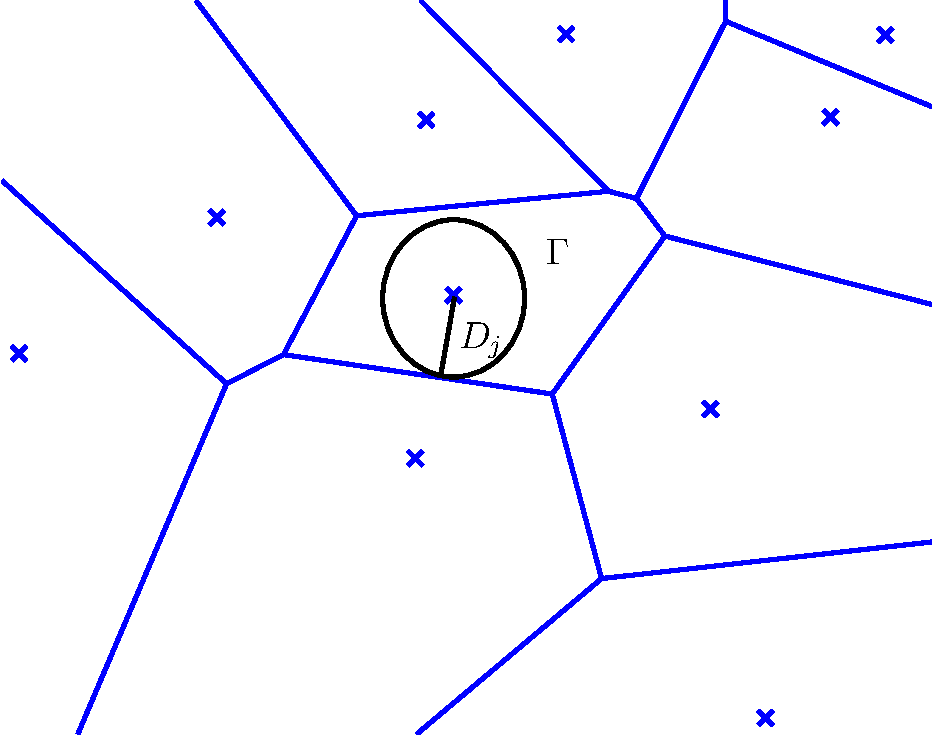
\includegraphics[width=0.6\textwidth]{voronoi.pdf}
    \end{center}
\end{frame}
\subsection{Séparation des cellules}
\begin{frame}{Séparation des cellules}
    On définit le potentiel « longue distance », qui, à l'intérieur d'une cellule, ne « voit pas
    » le noyau associé. Dans $\Gamma_i$,
    \[\Phi(x) = \alpha z \sum_{j\neq i} \frac{1}{|x-R_j|}.\]
\end{frame}
\newcommand{\vv}{\widetilde{V}}
\newcommand{\vvv}{\widehat{V}}
\begin{frame}{Séparation des cellules}
    On sépare l'énergie potentielle :
    \[V = \vv + \Phi,\]
    avec
    \[\vv(x) = \frac z {|x - R_i|} \text{ dans $\Gamma_i$}\]
    \begin{align*}
    \mathcal{E} =&
    \overbrace{a^2\int (\nabla \rho^\frac{1}{3})^2 + b^2 \int \rho^{4/3}
    - \int \vv \rho}^{\mathcal{E}_1}\\
    &\overbrace{-\int \Phi \rho +  \frac{\alpha}{2}\int\frac{\rho(x) \rho(y)}{|x-y|}+U,}^{\mathcal{E}_2}
    \end{align*}
\end{frame}

\begin{frame}{Inégalité électrostatique de Lieb et Yau}

    Contrôle de l'énergie potentielle longue distance
    par l'interaction électronique et l'interaction nucléaire.

    \vspace{1cm}

    Pour toute densité $\rho$,
    \[\int\Phi(x)\rho(x) \leq \frac{\alpha}{2}\iint
    \frac{\rho(x)\rho(y)}{|x-y|} + U -
    \alpha \frac{z^2}{8}\sum_j \frac{1}{D_j}.\]
\end{frame}

\begin{frame}{Interaction inter-cellulaire}
  \begin{align*}
    {\mathcal{E}_2} = {-\int \Phi \rho +  \frac{\alpha}{2}\int\frac{\rho(x) \rho(y)}{|x-y|}+U,}
  \end{align*}
  On contrôle $\int \Phi \rho$ avec l'inégalité électrostatique
  \begin{align*}
        \mathcal{E}_2 \ge& \frac{\alpha z^2}{8}\sum_j \frac{1}{D_j}.
  \end{align*}

\end{frame}
\begin{frame}{Interaction intra-cellulaire}
  \begin{align*}
    \mathcal E_1 = {a^2\int (\nabla \rho^\frac{1}{3})^2 + b^2 \int \rho^{4/3}
    - \int \vv \rho}
\end{align*}

Contrôle de $\int \vv \rho$ ?

Si $\vv$ n'était pas singulier, on pourrait utiliser H\"older
  \begin{align*}
    \int \vv \rho \leq \Vert\vv\Vert_{4} \Vert\rho\Vert_{4/3}
  \end{align*}
  pour faire apparaître $(\int \rho^{4/3})^{3/4}$ et conclure.

  Problème: $\vv \not \in L^{4}$.

  On sépare la partie singulière

\end{frame}

\subsection{Isolation de la singularité}
\begin{frame}{Isolation de la singularité}
  \begin{align*}
    \mathcal E_1 = {a^2\int (\nabla \rho^\frac{1}{3})^2 + b^2 \int \rho^{4/3}
    - \int \vv \rho}
\end{align*}
  Contrôle de $\int \vv \rho$

  \begin{align*}
    \int \vv \rho &= \sum_j \underbrace{\int_{B_j} \vv
      \rho}_{\text{?}} + \sum_j \underbrace{\int_{\Gamma_j -
      B_j} \vv \rho}_{\text{Hölder}}
\end{align*}
\end{frame}

\definecolor{gris}{rgb}{.2 .2 .2}
\begin{frame}{Principe d'incertitude modifié}
  Contrôle de la singularité coulombienne dans toute boule (et non pas
  sur tout l'espace comme dans le cas atomique)

    \vspace{1cm}

    Pour toute densité $\rho$ :
    \begin{align*}
      \frac {4ab}{3} \int_{B_j}
       \frac 1 {|x|}\rho(x)\dd x &\leq
      a^2\int_{B_j}\left|\nabla \rho(x)^{\tiny{\frac{1}{3}}}\right|^2 \dd x + b^2 \int_{B_j} \rho(x)^{4/3}\dd x \\&+ \frac{2ab}{R} \int_{B_j}
    \rho(x)\dd x.
    \end{align*}

\end{frame}


\begin{frame}{Contrôle de la singularité}
On contrôle $\int_{B_j} \vv \rho$ par le P.I.M. si
\begin{align*}
  \alpha z \leq \frac{4ab}{3}
\end{align*}

Mais on veut garder du $\int \rho^{4/3}$ pour $\int_{\Gamma_j - B_j}
\vv \rho$:
\begin{align*}
  b^2 &= b_1^2 + b_2^2,\\
  \alpha z &= \frac{4ab_2}{3}
\end{align*}
\end{frame}
\begin{frame}[fragile]{Contrôle de la partie non singulière}
  \begin{align*}
    \mathcal{E}_1&\geq
    b_1^2 \int \rho^{4/3} - \sum_j \int_{B_j}\frac{3\alpha z}{2 D_j} \rho
    - \sum_j\int_{\scriptscriptstyle\Gamma_j\setminus B_j} \vv \rho\\
    &\ge
    b_1^2 \int \rho^{4/3} - \int_{\mathbb{R}^3} \vvv\rho,
  \end{align*}
  où

  \begin{minipage}{0.2\linewidth}
    \centering
    \small
    \begin{align*}
      \vvv(x) &= \left\{\begin{aligned}
          \frac{3\alpha z}{2D_j} && x \in B_j\\
          \frac{\alpha z}{|x-R_j|} && x \in \Gamma_j \setminus B_j\end{aligned}\right.
    \end{align*}
  \end{minipage}
  \begin{minipage}{0.5\linewidth}
    \centering
    \begin{asy}
import graph;
size(5cm);
real i=0.5;
real f(real x) {return 1/abs(x);}
real g(real x) {return 1/i+1;}
draw(graph(f,i,4),blue+3*linewidth(currentpen));
draw(graph(g,0,i),blue+3*linewidth(currentpen));
xaxis('$|x-R_j|$');
yaxis('$\widehat{V}$');
labelx('$D_j$',i);
draw((i,g(i))--(i,0),dashed);
\end{asy}
\end{minipage}

$\vvv$ n'est plus singulier, on peut le contrôler par Hölder.
\end{frame}

\begin{frame}{Contrôle de la partie non singulière (2)}
            \begin{align*}
                \int \vvv \rho \le& \Vert\vvv\Vert_4 \Vert\rho\Vert_{4/3},\\
                \intertext{donc}
                \mathcal{E}_1 \ge&\,b_1^2 \int \rho^{4/3} -
                \Vert\vvv\Vert_4 \left(\int \rho^{4/3}\right)^{3/4}\\
                \ge& b_1^2 X - \Vert\vvv\Vert_4 X^{3/4}
                \intertext{En optimisant sur $X$ on a :}
                \mathcal{E}_1 \ge& -\frac{1}{4}\left( \frac{3}{4b_1^2}
                \right)^3\Vert \vvv \Vert_4^4.
              \end{align*}
              On calcule
              \begin{align*}
                \int \vvv^4 \leq \sum_j \frac 1 {D_j} (\alpha z)^4 (\underbrace{\frac 4 3 \pi}_{B_j}
                  +  \underbrace{{3 \pi}}_{\mathbb R^3 \setminus B_j})
              \end{align*}
\end{frame}
\subsection{Conclusion}
\begin{frame}{Conclusion}
  Finalement, si $b_2(z) < b$,
  \[\mathcal{E} \ge M(z) \sum_j \frac{1}{D_j}\]

  On en déduit une condition sur $z$ et le résultat
        \[\mathcal{E}\ge 0\quad\text { si }\quad \max z_i \le \frac{4ab}{3\alpha}\sqrt{1-x},\]
        \medskip
        où $x$ est solution de
        \[\frac{1-x}{x^3}=\frac{b^4}{a^2}\left( \frac{4}{3}
        \right)^2\frac{1}{2\pi\alpha(4+9\alpha^4)}.\]

\end{frame}
\section{Conclusion}
\begin{frame}{Conclusion générale}
  \begin{itemize}
  \item Cas atomique : preuve par réarrangement symétrique
  \item Cas moléculaire : condition de stabilité sur $\max z_i$
  \item On se ramène à un cas quasi-atomique dans les cellules du
    diagramme de Voronoï
  \item Résultat presque aussi bon que dans le cas atomique
  \item On peut montrer le même résultat d'instabilité que dans le cas
    atomique en concentrant $\rho$ sur un atome
  \end{itemize}
\end{frame}
\begin{frame}{Points pour discussion et questions ouvertes}
  \begin{itemize}
  \item Origine du modèle
  \item Argument de concavité
  \item $z_c$
  \item ...
  \end{itemize}
\end{frame}
\end{document}
